\documentclass[tikz,border=4pt]{standalone}
\usepackage{tikz}
\usetikzlibrary{arrows.meta, positioning, shapes.geometric}

\definecolor{mutblue}{RGB}{30,90,210}

\begin{document}
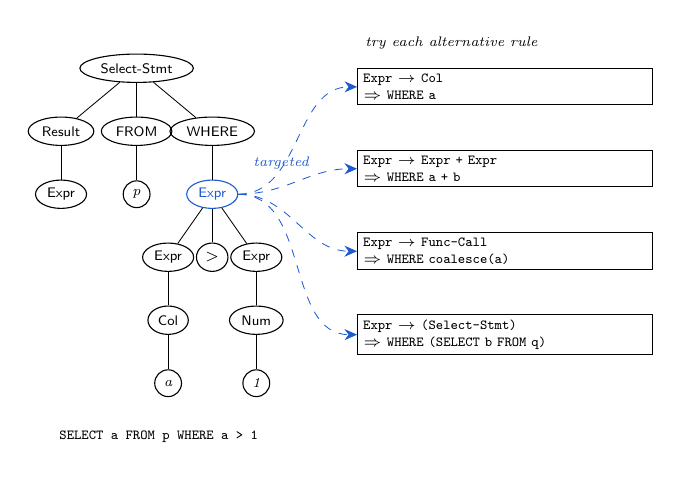
\begin{tikzpicture}[
    x=8mm, y=8mm,
    every node/.style={font=\tiny},
    nt/.style={ellipse, draw=black, line width=0.4pt,
        inner xsep=1.5pt, inner ysep=1pt, font=\tiny\sffamily,
        minimum height=3.6mm},
    op/.style={ellipse, draw=black, line width=0.4pt,
        inner xsep=0.5pt, inner ysep=1pt, font=\tiny\sffamily,
        minimum width=4mm, minimum height=3.6mm},
    lf/.style={circle, draw=black, line width=0.4pt,
        inner sep=0pt, minimum size=3.4mm, font=\tiny\itshape},
    nth/.style={ellipse, draw=mutblue, line width=0.4pt,
        inner xsep=1.5pt, inner ysep=1pt, font=\tiny\sffamily,
        minimum height=3.6mm, text=mutblue},
    te/.style={draw=black, line width=0.3pt},
    varbox/.style={rectangle, draw=black, line width=0.4pt, align=left,
        inner sep=2pt, text width=36mm, font=\tiny\ttfamily,
        anchor=north west},
    dasharrow/.style={-{Stealth[length=1.6mm,width=1.4mm]}, dashed,
        line width=0.3pt, draw=mutblue},
]

% ===== LEFT: input tree =====
\node[nt] (root)   at (0,0)    {Select-Stmt};

\node[nt] (result) at (-1.2,-1) {Result};
\node[nt] (from)   at (0,-1)    {FROM};
\node[nt] (where)  at (1.2,-1)  {WHERE};

\node[nt]  (expr1)  at (-1.2,-2) {Expr};
\node[lf]  (p)      at (0,-2)    {p};
\node[nth] (target) at (1.2,-2)  {Expr};

\node[nt] (lexpr) at (0.5,-3) {Expr};
\node[op] (gt)    at (1.2,-3) {$>$};
\node[nt] (rexpr) at (1.9,-3) {Expr};

\node[nt] (col)   at (0.5,-4) {Col};
\node[nt] (num)   at (1.9,-4) {Num};

\node[lf] (a)   at (0.5,-5) {a};
\node[lf] (one) at (1.9,-5) {1};

\foreach \a/\b in {root/result, root/from, root/where,
    result/expr1, from/p, where/target,
    target/lexpr, target/gt, target/rexpr,
    lexpr/col, rexpr/num, col/a, num/one}
    \draw[te] (\a) -- (\b);

% "targeted" caption: placed above-right of target between WHERE and target,
% in clear space (no edges or arrows go through here).
\node[font=\tiny\itshape, text=mutblue, anchor=west]
    at (1.7,-1.5) {targeted};

\node[font=\tiny\ttfamily, anchor=north] at (0.35,-5.6)
    {SELECT a FROM p WHERE a > 1};

% ===== RIGHT: rule alternatives =====
% Place boxes to the right of the tree, at x=3.5 (= 28mm from origin)
\node[font=\tiny\itshape] at (5.0,0.4) {try each alternative rule};

\node[varbox] (v1) at (3.5, 0)
    {Expr $\to$ Col\\$\Rightarrow$ WHERE a};
\node[varbox] (v2) at (3.5, -1.3)
    {Expr $\to$ Expr + Expr\\$\Rightarrow$ WHERE a + b};
\node[varbox] (v3) at (3.5, -2.6)
    {Expr $\to$ Func-Call\\$\Rightarrow$ WHERE coalesce(a)};
\node[varbox] (v4) at (3.5, -3.9)
    {Expr $\to$ (Select-Stmt)\\$\Rightarrow$ WHERE (SELECT b FROM q)};

\draw[dasharrow] (target.east) to[out=0,in=180] (v1.west);
\draw[dasharrow] (target.east) to[out=0,in=180] (v2.west);
\draw[dasharrow] (target.east) to[out=0,in=180] (v3.west);
\draw[dasharrow] (target.east) to[out=0,in=180] (v4.west);

\end{tikzpicture}
\end{document}